\documentclass{article}
\usepackage{graphicx}
\usepackage{amsmath}
\usepackage{amsfonts}

\begin{document}
\section*{Doppelspalt}
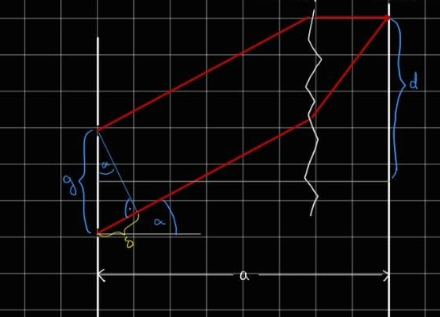
\includegraphics[width=\textwidth]{dp.png}
\begin{align}
    a = \text{Abstand zum Schirm} \\
    g = \text{Spaltabstand} \\
    d = \text{Distanz zur Schirmmitte} \\
    \delta := \text{Gangunterschied}
\end{align}
\subsection*{Idealisierungen}
\begin{enumerate}
    \item Die Spalte betrachten wir als punktförmig. Daher ist jeder Spalt Ursprung iner Elementarwelle und der Gangunterschied beträgt
    $\delta = |s_1 - s_2|$
    \item Der Schirm hat einen sehr großen Abstand im  Vergleich zum Spaltabstand $(a>>g)$. Das bedeutet, das wir beide Wellen als
    parallel ansehen können.
    \item Für kleine Winkel $(\alpha < 5^\circ)$ gilt $tan(\alpha)\approx sin(\alpha)$
\end{enumerate}
\subsection*{Formeln}
\begin{align*}
    sin(\alpha)=\frac{\delta}{g}\\
    tan(\alpha)=\frac{d}{a}\\
    \text{Dritte Idealisierung:}\\
    d = \frac{\delta a}{g}\\
    \text{Inteferenzmaxiumum}\\
    d = \frac{k*\lambda*a}{g} (k\in \mathbb{N})\\
    \text{Inteferenzminimum}\\
    d = \frac{(2k-1)*\lambda*a}{g} (k \in \mathbb{N}\text{\textbackslash}\{0\})
\end{align*}
\section*{Inteferenz am Gitter}
Für ein schärferes Inteferenzbild nutzt man meist ein optisches Gitter.
Die Gitterkonstante \emph{g} steht für den durschschnittlichen Abstand zwischen Gitterlininen.
Die Maxima sind scharf begrenzt, da sich bereits für geringe Gangunterschiede Partnerspalte wirken, die destruktiv
inteferieren. Da die Maxima durch die konstruktive Inteferenz vieler Strahlen entstehen, sind sie intensiver
\subsection*{Idealisierungen}
\begin{enumerate}
    \item Punktförmige Spalte bilden die Ausgangspunkte von Elementarwellen
    \item Da der SChirmabstand viel größer als der Spaltabstand ist, können die Wellenstrahlen als parallel angesehen werden.
    \item Es treten Winkel über 5\textdegree auf. $sin(\alpha)=tan(\alpha)$ kann daher nicht verwendet werden.
\end{enumerate}
\subsection*{Formeln}
\begin{align*}
    \text{Im Abstand dk befindet sich das k-te Maximum}\\
    tan(\alpha)=\frac{d_k}{a}\\
    \text{Für den Gangunterschied des k-ten Maximums gilt}\\
    sin(\alpha)=\frac{\delta}{g}=\frac{k*\lambda}{g}\\
    \text{Maximalzahl an Maxima 2*k+1 (da max. 90 Grad):}\\
    sin(90)=\frac{k*\lambda}{g} \geq 1\\
\end{align*}

\end{document}